%
% $Id: ch01_overview
%
%   *******************************************************************
%   * SEE THE MAIN FILE "AllegThesis.tex" FOR MORE INFORMATION.       *
%   *******************************************************************

\chapter{Introduction}\label{ch:intro} % we can refer to chapter by the label
Software systems are very complex in nature and because of this fact, they are very difficult to test. As Fred Brooks Jr. has said, ``Software entities are more complex for their size than perhaps any other human construct because no two parts are alike (at least above the statement level).''~\cite{brooks1987no} As a system grows, the interactions that each module has to the system becomes increasingly complex. Modules can become so interconnected that it may be hard to keep track of how different pieces of a system interact with each other let alone their functionality. Since many systems can be separated into modules and shared to other parts of the program, it is important to understand whether a system is working as intended by the  developer. To verify if the system has been implemented correctly, developers often look to testing.

% * What is Testing (DEF)
Software testing is a verification process for software quality assessment and software quality improvement~\cite{friedman_voas_1995}. The first way to check whether or not a system is functioning properly is to ask a simple question, ``Is it currently operating or has it crashed?'' Performing an eyeball examination of a system is a very helpful step in the process of verification. However, if the system is not crashed and there is no significant data incorrectness, it could be very easy to miss a system that is not operating properly. That is why eyeball examination, for the most part, has been replaced with Unit testing.

%   * What is Unit Testing
Unit testing is the process of testing different modules of the system in isolation~\cite{friedman_voas_1995}. This could entail taking one function, observing its inputs, and then testing it with an outcome that is understood and accepted. A simple example would be a function that takes in two numbers, \texttt{X} and \texttt{Y}, and multiplies them together. The test case would supply the numbers 2 and 3 to the function, and then assert that the result is 6. This example was written in the Python language with the Pytest framework and is illustrated in Listing \ref{testingExample}.

%       * Unit Testing Example
\begin{figure}[t!]
\begin{lstlisting}[language = Python, numbers = left, frame = single, caption = Example of a unit test in the Pytest~\cite{okken_2018} framework., label = testingExample]
calulator.py:
  def multiplication(x,y):
    product = x*y
    return product


test_calculator.py:
  def test_multiplication():
    x = 2
    y = 3
    multiplicationResult = multiplication(x,y)
    assert multiplicationResult == 6
\end{lstlisting}
\end{figure}

%   * Ensuring that the system is running the way that it is intended
The way that testing ensures that a system is running correctly is by passing or failing cases in a test suite, or a collection of test cases. A developer will write a test case that is meant to have a desired effect, and if the system produces something that is unexpected the test will fail. The developer can write multiple test cases that have different inputs to observe how the system behaves under differing conditions. Each test can have a different intended purpose, in the case of \ref{testingExample}, the developer can write a test case that provides a null variable or a zero to see if the system can detect those two issues and resolve them in the intended manner. The variations that a test can take changes depending upon the intended functionality of the method it is testing.

% * coverage
One of the most important questions is, ``How can I know that my test suite is of good quality?'' As of right now, the answer to that question is coverage.

%   * What is coverage
Code coverage is a measurement of what percentage of the code under scrutiny is being tested by a test suite~\cite{okken_2018}. This metric can be used to ensure that developers are writing enough test cases for their systems. It reveals how much of the system is not being observed by the test suite.

%   * How is coverage calculated
This metric can be calculated in a variety of different ways, each one of which serves its own purpose.
%     * Branch
Branch coverage is the  percent of all control sequences being completed during the testing of the system~\cite{zhu1997software}. Simply put, branch coverage is looking to observe if every path of decision trees is being executed during the test run. So if there is an if/else statement that is checking if a number is even or odd, the test suite needs to include a test case for each of these scenarios.

%     * Branch coverage calculation
        \begin{quote}
        \textbf{\textit{Definition:}} Branch coverage is the fraction of the total number of branches that have been executed by the test data~\cite{malaiya2002software}.

        \begin{equation}
        \mbox{\emph{Branch Coverage}} = \frac{\mbox{\emph{Tested Branches}}}{\mbox{\emph{Total Number of Branches}}}
        \end{equation}
        \end{quote}

%     * statement
Statement coverage is the most brute force code coverage metric. It is the  percent of statements that have been executed in the test suite. So if there are 100 statements in the system, and only 85 are being executed, the coverage check will reward the system with being 85 percent covered.

%     * Statement coverage calulation
\begin{quote}
\textbf{\textit{Definition:}} Statement Coverage is the fraction of the total number of statements that have been executed by the test data~\cite{malaiya2002software}.

\begin{equation}
\mbox{\emph{Statement Coverage}} = \frac{\mbox{\emph{Tested Statements}}}{\mbox{\emph{Total Number of Statements}}}
\end{equation}
\end{quote}
%     * function
One of the most useful types of coverage is the function coverage. This is the percentage of the functions in the system that have been executed in a test case. This is a very baseline example for the unit testing as mentioned before. Testing of each function helps developers know if the intended behavior within the functions that are helping the system run are performing as intended. The following equation is used to calculate this type of coverage:

%     * function coverage calculation
        \begin{quote}
        \textbf{\textit{Defintion:}} A method \textit{m} $\in$ \textit{P} is said to be covered if there exists at least
        one test case \textit{t} $\in$ \textit{TS}, the test suite of program \textit{P} that triggers the execution of at least one path of the
        body of \textit{m}. \textit{TS} is the test suite of \textit{P}~\cite{vera2017comprehensive}.

        Where (\textbf{\textit{TM}}) is the number of tested methods in \textit{P},

        \begin{equation}
        Function Coverage = \frac{TM}{NUMM}
        \end{equation}
        \end{quote}

%   * Why is coverage helpful
Checking the code coverage is a very important step in the development of a large scale system. It can help a developer understand what code needs to be tested, and ensures that there is at least one test case for every function. The need for a system with high coverage is important, but it does raise a very important question, ``Is there a way for a developer to know if they have a good test suite?''

%   * Why can coverage be misleading
Coverage is a very important measure, but it can be misleading. It is helpful to show a developer how much of their system has been covered by the test suite, but it does not provide any information on the test suite having high fault detection effectiveness. A test case that has a call to a function, but cannot detect a bug will still be counted as covered if the calculation was running under function coverage. ``Although 100\% branch coverage will make us feel better about the reliabilty than will 50 percent branch coverage, the true reliability of the code will be the same.~\cite{friedman_voas_1995}'' Parts of the system that are not being tested could include bugs that the developers have not yet found, or that the developer is not testing for. The subject that coverage leaves out of its calculations is pseudo-tested methods.

% * Pseudo-tested methods
%   * What is a pseudo-tested method and why is it an silent issue
A pseudo-tested method is a method that will still pass test cases when the effects of a method are suppressed~\cite{vera2017comprehensive}. Simply put, it is a test case that will never fail. A pseudo-tested method can heavily impact a system. If there is unexpected information given to a pseudo-tested method and it doesn't know how to handle it, either bad results will follow or the system could crash. The only indicator that a pseudo-tested method has been written is that a test will never fail, regardless of the inputs that it is taking. The issue with this indicator is that passing test cases is a good thing. Many developers will overlook a passing test case, simply because it is passing. This makes sense, it follows the idea of, ``if it isn't broken, don't fix it.'' Therein lies the problem with pseudo-tested methods. Why would a developer investigate something that does not indicate a problem in what they wrote? This is an interesting concept because the way that a pseudo-tested method can exist is by writing a test case that will never fail.

%   * They are really easy to write
It seems as though it would be difficult to write a test case for a method that will never fail, but it is actually very easy. Whether it comes from developer error or not testing for the right things, it is entirely possible to write this type of test case.
%   * What does a pseudo-tested method look like
A pseudo-tested method could be produced in a variety of different forms, but a version of human error is represented in Listing \ref{pseudo}. To explain the example, the method \texttt{numberCheck} is being pseudo-tested. The test is checking whether or not the function \texttt{numberOrder} is sorting a list of numbers that is given to it.  Unfortunately the test, whether or not intended, is testing the initial set of numbers when it should be testing the list of sorted numbers with what is returned. More importantly the test is using sets and not lists. In sets the order does not matter, in lists order is maintained. Therefore the test will never fail, even though a list of numbers that is not ordered is being compared to a list of numbers that is ordered. This example serves to show how simple it is to accidentally pseudo-test methods. This test is not analyzing the correct variable and is not using the correct datatype, but the test will never fail.

%   * Pseudo-tested method example
\begin{figure}[t!]
\begin{lstlisting}[language = Python, numbers = left, frame = single, caption = Example of a pseudo-tested method, label = pseudo]
numbers.py:
  def numberOrder(n):
    numbersSorted = sorted(n)
    return numbersSorted


test_numbers.py:
  def test_numbers_ordered():
    numbers = set([1,3,2,4])
    sortedNumbers = set([1,2,3,4])
    orderedNumbers = numberOrder(numbers)
    assert numbers == sortedNumbers
\end{lstlisting}
\end{figure}

Pseudo-testing as an action is the product of unknowingly creating a test that will always be satisfied. There are many reasons that this can occur, and this is a problem that exists in larger systems as well. Even large systems that maintain a very high coverage contain many pseudo-tested methods~\cite{vera2017comprehensive}. As stated before, this is because the metric that many of these larger systems rely on, coverage, could be a misleading metric. What are the circumstances for a pseudo-tested method to be created? One is a company that is expected to maintain a high level of code coverage. This could lead to employees writing a test case just to write a test case and fulfill the baseline requirements so that they may have their pull requests approved. This is an industry-wide issue as many companies will not allow pull requests if the test coverage is any lower than 100 \%\cite{prause2017100}. The other issue is having a test case pass and simply moving along without any further examination. If a developer does not know that they have written a pseudo-tested method, and has a passing test case, they may begin development somewhere else. Since this test would be considered covered, it would also be included in pull requests further affecting different portions of the system.

Since it is so easy to write a pseudo-tested method, what are the current ways for automatic detection of pseudo-tested methods? The short answer for the Python programming language is that there isn't one. There are really only two ways for determining the fault detection effectiveness in Python, and both are by hand. Observing that the inputs and outputs of the functions can become tedious by hand provides the possibility that there could be inputs that will still fail the test suite, but not be tested. The other way is to do a proof of correctness for the test suite. The main issue with this type of validation is that it can take a very long time, and by the time that there is a pseudo-tested method found, the functionality of that portion of the system could have changed. Even visually it is very hard to notice pseudo-tested methods if the developer is not specifically looking for them.

Since initially there was no way to detect pseudo-tested methods automatically or manually with any accuracy, this thesis introduces the Automatic Detection Tool: Function-Fiasco.

Function-Fiasco is a tool that analyzes Python programs that are tested with the Pytest framework~\cite{okken_2018} to automatically detect pseudo-tested methods. It will check every method that is in the program by supressing the behavior of the system to determine if the test is strong enough to detect when there are unexpected changes to the way the method works. Function-Fiasco uses a combination of fault-injection, fuzzing, and mutation testing to accurately assess a system's test suite to detect pseudo-tested methods. Function-Fiasco supports primitive data types to return a table that describes the coverage of the system as a percent of the amount that is covered, and represents the fault detection effectiveness.

Function-Fiasco was used on a group of 10 GitHub projects to determine its effectiveness and the amount of pseudo-tested methods that are present in Python based systems. The important contributions of this research are as follows:

\begin{enumerate}
  \item A working automatic detection tool for pseudo-tested methods for Python based systems.
  \item A table that contains the results of a system's coverage and fault detection effectiveness.
  \item A revised metric that describes how accurately a system is able to detect errors.
  \item Two Pytest plugins that aid in the testing of software.
\end{enumerate}

%
\section{Motivation} \label{sec:motivation}
%
% * Why testing is so important in general
Function-Fiasco was created because testing as a topic is very important. Testing is the way that developers will know how a certain condition will affect a system. A well tested system is stable and prepared for any unexpected changes to function inputs. This is the main reason that testing exists on every software engineering model. Without testing, developers would not know the true behaviors of the system and may have written a bug that could crash during execution or provide incorrect results to a user. While designing a system is a very important part of the development cycle, designing the test suite that it will be running beside and verifying its functionality could arguably be more important. Developers use test suites to ensure that the work that they are doing is correct and intended. This process can be broken into two different pieces. Validation is the process of ensuring that the sofware is doing the right thing and verification is the process of ensuring that the software is performing its purpose correctly~\cite{friedman_voas_1995}. In the past, much of the software assessment would be completed towards the end of the cycle. Function-Fiasco is still able to help systems that are being tested in this manner as it will help developers know if they are writing tests that will detect bugs. There has been a recent push towards a more \textit{test-first} mindset. Test-driven development is a rising idea in Software Development. In test-first development, the system is thought out and test cases are written prior to the writing of the software. Test-first development has many benefits, such as a greater organization and a better understanding of the flow of the system. Additionally, developers know when they have created software that fits the intended functionality of the system~\cite{fucci2017dissection}. Function-Fiasco is also able to help in Test-driven development. After a test has been written in the process of Test-driven development, functionality implementation begins. This is the process of understanding what a function needs to do and writing the implementation that will complete this process. Tests are often used to determine if a developer has written the right implementation. Function-Fiasco can be used at this stage. It can be used to determine if the tests will be able to detect all mutations that the code can take.

% * Has not been done in python before
The second most important reason for the creation of this tool is that nothing like it exists for the Python programming language. One other tool Descartes is a tool that automatically detects pseudo-tested methods in the Java programming language for systems~\cite{vera2018descartes}. This is the only other tool that analyzes systems for pseudo-tested methods, and since it is made for the Java programming language, it will not work on systems of other programming languages. Also, it has been explained that mutation testing results can be skewed by the programming language~\cite{vera2017comprehensive}. This can be explained by the different algorithms that different programming languages use and the idea of type safety. Programming languages, such as Java, that use strict typing will not overwrite a variable with a different type, like an \texttt{int} becoming a \texttt{char}. Python will perform such an operation, an example of this is in Listing 1.3, where the new value of \texttt{a} is the \texttt{String} instead of the \texttt{int}. The reasoning is Python does not require declarations to reserve memory space. Therefore there needs to be a tool that will detect pseudo-tested methods in Python.
% * needed metric for code testing

The next piece of motivation is the potential misleading nature of coverage. As mentioned before, as long as a function is called in a test suite, that function is considered covered. Coverage cannot give an indication of the fault detection effectiveness for a test suite, which is a very important part of testing. If there is no way to determine that a test suite is properly created, and developers have to rely solely on coverage as a validation metric, the easy creation of pseudo-tested methods will remain. One of the only ways to determine the fault detection effectiveness of a test suite is to do a check on each test case by hand and to run many different mutations for it. This type of work can be very time consuming and would create a unneccessarily long list of test cases that can become redundant. That is why many companies lean towards using coverage, as it implies that many mutations are covered in the test suite, when in reality it is only how much of the program is being executed in the test suite. Function-Fiasco generates a metric that is the overall coverage which is modified to reflect the number of pseudo-tested methods. This metric is representative of the overall behaviors in the system. It will allow developers to not only know how much of their system is covered, but it will also give them an idea to the fault detection effectiveness of their test suite.

\begin{figure}[t!]
\begin{lstlisting}[language = Python, numbers = left, frame = single, caption = Example of interpreted languages, label = interpreted]
inter.py:
  print("1")
  print("2")
  print("3")

\end{lstlisting}
\end{figure}

% * What is python?
The final reason that Function-Fiasco was created, is for the Python language. Python is quickly becomming one of the most popular languages in terms of job opportunities as shown in Figure \ref{languageGrowth}~\cite{wang2017computer}, which was generated using the Indeed Job Trends. Python is an interpreted, interactive, object-oriented programming language\cite{sanner1999python}. An interpreted language is a language that is compiled during runtime for errors, such as syntax. An example is Listing \ref{interpreted}. In this example, both the numbers 1 and 2 will print during the execution of the program. Then the system will encounter the incorrect syntax of the \texttt{print} statement and crash. Python is also a very loosely typed language, which means that variables can easily be overwritten. This loose type safety directs to the hypothesis of: \emph{Since Python is a loosely typed language, there could potentially be a higher concentration of pseudo-tested methods written into systems that are written in Python.} Another factor in in the choice for Python, was the Pytest framework. The reason that Python was the chosen language for Function-Fiasco is the growing popularity of the language.  Since it is becomming more popular and Python has loose type safety, there needs to be a tool that makes it easier for developers to know when they have written test cases that represent the fault detection effectiveness, and Function-Fiasco helps accomplish that. Function-Fiasco will indicate that test cases are still passing when they shouldn't. For example, if a developer is accidentally using the wrong datatype, as shown in Listing \ref{pseudo} and the test still passes, Function-Fiasco will be able to detect that.
\begin{figure}[htbp]
  \centering
  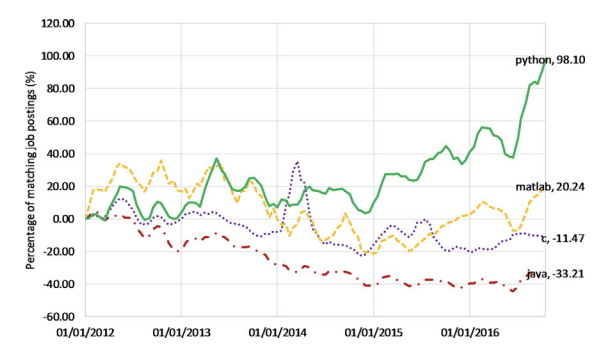
\includegraphics[width=5in]{images/language-growth.png}
  \caption{Job opportunities per language~\cite{wang2017computer}.}~\label{languageGrowth}
\end{figure}




%   * Explain the benefits of python
% * More valuable
% * why did I choose it


\section{Current State of the Art}\label{sec:stateofart}

As mentioned previously, the current state of the automatic detection for pseudo-tested methods is almost non-existant. Other than Function-Fiasco, there are three ways to detect a pseudo-tested method. Decartes is a tool that uses mutation testing to detect pseudo-tested methods, but this tool could only assist a developer if they are using Java. Descartes will not assist developers in any other programming language. Mutation testing is the process of changing code to produce a mutant that will be detected by the test case. If the mutant is not detected, a mutation score is calculated by using the ratio of detected mutants to total mutants. This score is representative of the test suite effectiveness. This score can be calculated as follows:

\begin{quote}
\begin{equation}
\mbox{\emph{Mutation Score}} = \frac{\mbox{\emph{Detected Mutants}}}{\mbox{\emph{Total Mutants}}}
\end{equation}
\end{quote}

It is important to note that the way that Function-Fiasco employs mutation testing is vastly different from Descartes. Decartes uses extreme mutations. Extreme mutation very simply removes all side effects of a function from the running of a system. In Decartes, if a function has a void return, all statements will be removed from the body of the function. If there is a return type, a pre-determined value is returned. This complete change is meant to be caught by the test suite. If it is not, the function is pseudo-tested~\cite{vera2018descartes}. Function-Fiasco does not affect the statements inside the body of a function at all. However, it does interact with functions, but only so that it may add decorators to indicate to Function-Fiasco where a mutation needs to occur. It will then allow the function to be run. This is so that it may determine the return type of the system, this is necessary as Python is a loosely-typed language. It will then randomize the value of the return so that the test suite is receiving an input that is not what was expected, but is of the correct type except in cases where a \texttt{boolean} is returned. So instead of a mutation of code structure or statements, there is a mutation of the inputs into the test suite.

The other way of detecting pseudo-tested methods is by checking each function by hand. A developer may look at a test suite to determine its inputs and expected output and run a visual test. This test will check if inputs that are known to produce a failing result will actually detect a failing result. If this result is passing, the function that is being tested is considered pseudo-tested. This process is very tedious and still has the impact of human error. Because a human is preparing the inputs that the test will receive, these tests may not be testing the right inputs, due to the potential for human error. For example, a test would pass if it receives a postive number, but the developer does not know that a negative number may pass as well. This developer can create five scenarios to test positive numbers, but never see that the test will pass even if it receives a negative number. The mutation for the inputs by a human always has an element for human error. One other significant issue with testing systems by hand is that the size and complexity of systems may make this work meaningless. Since this is a very time consuming task, depending on the size of the system, the functionality of the portion of the system that is being hand tested may change before the test determines if a function is being pseudo-tested.

The final way to detect for a pseudo-tested method is one that may sound dangerous, and it is: to not test for it at all. The idea of a pseudo-tested method is a relatively new topic. This is evident as the idea was introduced by Niedermayr and colleagues~\cite{niedermayr2016will}~\cite{vera2017comprehensive}. This means that there could be a plethora of systems in the field that have functions that are being pseudo-tested. This is a very frightening idea. Pseudo-tested methods are a relatively silent issue, which means that developers do not know about the dangers of them and are still writing them. Since many places are not testing for them at all, the way that the developers will realize that there is an issue with their test suite is when their system crashes or when certain results are not what was expected.

\section{Goals of the Project}\label{sec:goals}

% * there could be more pseudo-tested methods present in systems that are written using the python code base
%   * Prove that typed languages could contain less pseudo-tsted methods than typed languages
The first main goal of this research is to prove that there are pseudo-tested methods in systems that are written in loosely typed languages. The reasoning behind this goal is based around the syntax and semantics of strictly typed languages. For a loosely typed language, such as Python, variables can quickly be overwritten. So if a function is expecting a String, but it is given an integer, the system will not error, unless that variable is being used in a way that does not adhere to the data type. For a strictly typed language, this type of variable interaction will not be allowed. The system will produce an error, usually saying it was expecting a String, but received an int. Typed languages protect from interactions such as this, in a way forming a secondary test to ensure that the intended use of the function is followed. Loosely typed languages do not have this type of barrier, and may lead to the more concentrated creation of pseudo-tested methods.

% * explain the system that I have created to detect pseudo-tested methods in the pytest framework
This research was also meant to produce a tool that Python developers can use to ensure that the test suites they are creating have a high fault detection effectiveness. The tool can detect pseudo-tested methods automatically, which was not possible before. It was created in Python, for Python based systems that are being tested in the Pytest framework. Python was chosen because it is the fastest growing language and Pytest is one of the most popular testing frameworks, as indictated in Figure \ref{languageGrowth}. Function-Fiasco was meant to be used by the greatest number of people for the fastest growing systems, and is derived from multiple different testing techniques. These include: fault-injection, fuzzing, and mutation testing. This combination was intended to expose the systems that are being tested to the highest amount of observation so that pseudo-tested methods are detected. Afterwards, Function-Fiasco will deliver a table that is meant to serve as a report for the system.

% * create a metric that will allow developers in other languages to keep track of the fault detection effectiveness
The creation of a metric will allow developers to keep track of the fault detection effectiveness. One of the most significant issues in the field was that developers had to rely almost solely on coverage to determine if their test suite was of high quality. While it may have been in high quality for the amount of the system that was covered, as this is important information, it did not give any information on the fault detection effectiveness of the test suite. As a result, developers knew that a high amount of the system was tested, but had no indication as to how well it was being tested. Function-Fiasco provides a table that contains useful metrics that explain both the amount of the system that is being tested, as well as the fault detection effectiveness. Based upon this, developers in other languages have another metric that they can look to if they wanted to create a system that is able to determine the fault detection effectiveness.

% * Shed light on the silent issue
The final goal of this research was to shed light on the new concept that is pseudo-tested methods. Before 2016, there was almost no information on them. It is very important for an issue like this to get more acknowledgment from the computer science community. This is a problem that could potentially affect very large systems that are being used on a daily basis. There is only one other tool that has the capability to detect them, and two pieces of literature that agree that they exist. This research was completed to show that some of the current ways that we are testing systems can be improved to prevent them from being unstable.

\section{Thesis Outline}\label{sec:outline}
% The introductory chapter usually concludes with a ``road map'' of the upcoming
% chapters, e.g., ``Chapter \ref{ch:relatedwork} reviews a number of past approaches
% to the problem and summarizes their strengths and weaknesses. Chapter
% \ref{ch:method} outlines the method of approach used to establish the
% results.''

% why the content is in the order that it is
 This paper is organized as follows. Chapter \ref{ch:relatedwork} will discuss the past attempts at automatic detection and important resources that aided in the formulation of the tool, the past attempt being Descartes~\cite{vera2018descartes}. The other resources that will be mentioned include information on the Pytest framework, the research that founded the idea of pseudo-tested methods, as well as the paper that supported that research. The next chapter, Chapter \ref{ch:implem}, will describe the approach to how the system has been organized and how the functionality is created, as well as the decisions behind them. It will discuss how the Pytest is being run, as well as the decorator that is being used to determine the output of the functions. It will also describe the issues that arose during development. Chapter \ref{ch:method} will discuss the results of Function-Fiasco and what the different metrics mean. This includes the table that is created, the metrics that are found, and what they describe. It will also discuss the results of Function-Fiasco on numerous systems that can be found on GitHub. The final chapter, Chapter \ref{ch:conclusion}, will include discussionary topics and future work. As well as a brief summary of the results.
